\documentclass[a4paper,UTF8]{ctexart}

\usepackage{amsmath, amsthm, amssymb, amsfonts, hyperref, mathrsfs}%美国数学学会的包+?
\usepackage{geometry} %控制界面
\usepackage{bookmark}
\usepackage{fancyhdr} % header & footer
\usepackage{appendix} % 附录
\usepackage{tikz} %作图
\usepackage{graphicx} %插入图片的宏包
\usepackage{float} %设置图片浮动位置的宏包
%\usepackage{subfigure} %插入多图时用子图显示的宏包
\usepackage{listings} %引用代码
\usepackage{physics,mathtools} %物理数学工具
\usepackage{comment}
\usepackage{framed}
\usepackage{caption}
\usepackage{subcaption}
\geometry{top=2.5cm,bottom=2.5cm,left=2.5cm,right=2.5cm} % 布局要求
\pagestyle{fancy} % fancy分格
\fancyhf{} % 清除所有页眉页脚
\renewcommand\headrulewidth{0.6pt}
\renewcommand\footrulewidth{0.6pt}
\lhead{何金铭 PB21020660$\mid$座位号:2}
\chead{直流辉光等离子实验实验报告}
\rhead{\thepage}
\lfoot{2023.4.24}
\rfoot{USTC}
%\bibliographystyle{plain} % 引用样式
\everymath{\displaystyle} % display
%============================================================

\begin{document}

\begin{center}
    \textbf{\Large 直流辉光等离子实验实验报告}
    \par \text{\large 何金铭 PB21020660}
\end{center}

\section{实验目的}

\begin{enumerate}
    \item 观察直流低气压辉光等离子体的放电现象,通过对辉光等离子体的伏安特性
曲线的测量,理解辉光等离子体的电学特性;
    \item 理解直流电气击穿的机制;
    \item 验证帕邢定律;
    \item 采用 Langmuir 双探针法测量等离子体参数
\end{enumerate}

\section{实验原理}

\begin{comment}

\begin{figure}[H]
    \centering
    \begin{minipage}[b]{0.9\textwidth}
        \centering
        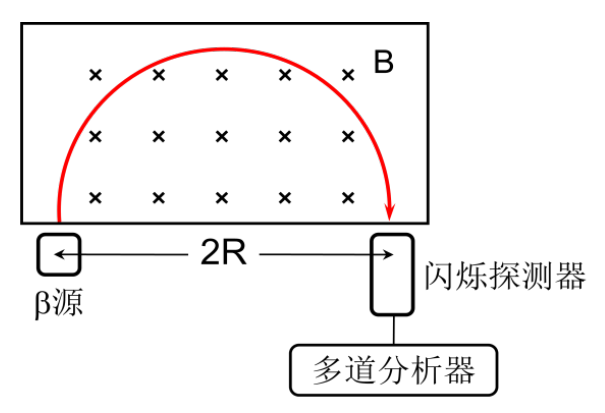
\includegraphics[width=0.4\textwidth]{./m.png}
        \caption{半圆聚焦$\beta$磁谱仪与闪烁能谱仪示意图}
    \end{minipage}
\end{figure}

\end{comment}

\subsection{等离子体及其物理特性及主要参量}

一般用来描述等离子体的参数有:

\begin{enumerate}
    \item 电子温度$T_e$。它是等离子体的一个主要参量,因为在等离子体中电子碰撞
电离是主要的,而电子碰撞电离与电子的能量有直接关系,即与电子温度相关联。
    \item 带电粒子密度。电子密度为$n_e$,正离子密度为$n_i$,在等离子体中$n_e \approx n_i$
    \item 轴向电场强度$E_L$。表征为维持等离子体的存在所需的能量
    \item 电子平均动能$E_e$
    \item 空间电位分布
\end{enumerate}

\subsection{气体放电}

气体放电可以采用多种能量激励形式,如直流、微波、射频等能量形式。其
中直流放电因为结构简单、成本低而受到广泛应用。

低气压放电可分为三个阶段:暗放电、辉光放电和电弧放电。其中各个阶段
的放电在不同的应用领域有广泛的应用。

\begin{figure}[H]
    \centering
    \begin{minipage}[b]{0.9\textwidth}
        \centering
        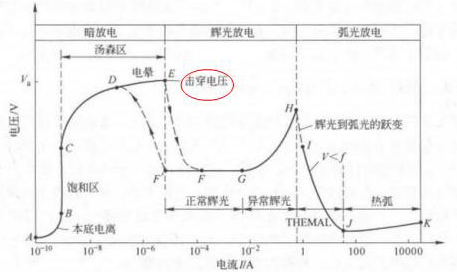
\includegraphics[width=0.9\textwidth]{./fig1.png}
        \caption{气体放电伏安特性曲线:AB 段—非自持放电本底电离区;BC 段—非自持放电饱和
区;CE 段—汤森放电区;DE 段—电晕放电区;EF 段—前期辉光放电区;FG 段—正常
辉光放电区;GH 段—异常辉光放电区;HK 段—弧光放电区}
    \end{minipage}
\end{figure}

\subsection{帕邢定律}

在低气压直流放电中,气体的击穿电压由下式决定:

\begin{equation}
    V_b = \frac{Cpd}{\ln{Apd/\ln{1+\frac{1}{\gamma}}}} = f(pd)
\end{equation}

其中$\gamma$为二次电子发射系数,常数 A、C 和气体种类有关的常数,p 为压强,
d 为阴阳极间距离,$V_b$为击穿电压。

上式表明某一特定气体的击穿电压仅仅依赖于pd 的乘积,这一现象被称为
帕邢(Paschen)定律。

\subsection{郎缪尔(Langmuir)探针}

探针是封入等离子体中的一个小的金
属电极(其形状可以是平板形、圆柱形、球形)。以放电管的阳极或阴极作为参
考点,改变探针电位,测出相应的探针电流,得到探针电流与其电位之间的关系,
即探针伏安特性曲线。

经过复杂且不重要的运算,可以得到以下结论

\begin{equation}
    T_e = -\frac{e}{k} \frac{I_{i01}I_{i02}}{I_{i01}+I_{i02}} (\frac{d\,V_D}{d\,I_D}\bigg|_{V_D = 0})
\end{equation}

其中$I_{i01},I_{i02}$分别为是探针 1、2 的离子饱和电流

\begin{equation}
    n_e = \frac{4I_{e0}}{eS_e} \sqrt{\frac{\pi m_e}{8k T_e}}
\end{equation}

其中$I_{e0} = 0.05A,S_e = 0.04cm^2$

利用实验数据绘制的双探针 V-I 特性曲线同理论曲线会有很大差距,绘制
V-I 特性曲线时要有足够的数据量,斜率 $\frac{d\,V_{D}}{d\,I_{D}}$ 取值要注意是在 $V_D = 0$ 附近,饱
和电流 $I_{i0}$ 一般用实验曲线中 $I_{i01}$ 和 $I_{i02}$ 延长线与纵轴的交点确定。

\section{实验仪器}

DH2006 型直流辉光等离子体实验装置

\section{原始实验数据}

\begin{table}[H]
    \begin{subtable}[h]{0.45\textwidth}
        \centering
        \begin{tabular}{| l | l|}
        \hline
        \textbf{电压/V} & \textbf{电流/mA} \\ \hline
        803 & 90 \\ \hline
        782 & 85 \\ \hline
        759 & 80 \\ \hline
        738 & 75 \\ \hline
        714 & 70 \\ \hline
        688 & 65 \\ \hline
        663 & 60 \\ \hline
        638 & 55 \\ \hline
        612 & 50 \\ \hline
        588 & 45 \\ \hline
        564 & 40 \\ \hline
        553 & 35 \\ \hline
        530 & 30 \\ \hline
        509 & 25 \\ \hline
        485 & 20 \\ \hline
        457 & 15 \\ \hline
        420 & 10 \\ \hline
        370 & 5 \\ \hline
        298 & 0 \\ \hline
       \end{tabular}
       \caption{P=20 Pa}
       \label{tab:p20}
    \end{subtable}
    \hfill
    \begin{subtable}[h]{0.45\textwidth}
        \centering
        \begin{tabular}{| l | l|}
\hline
        \textbf{电压/V} & \textbf{电流/mA} \\ \hline
        580 & 90 \\ \hline
        567 & 85 \\ \hline
        556 & 80 \\ \hline
        545 & 75 \\ \hline
        532 & 70 \\ \hline
        520 & 65 \\ \hline
        508 & 60 \\ \hline
        496 & 55 \\ \hline
        484 & 50 \\ \hline
        473 & 45 \\ \hline
        462 & 40 \\ \hline
        452 & 35 \\ \hline
        442 & 30 \\ \hline
        429 & 25 \\ \hline
        413 & 20 \\ \hline
        394 & 15 \\ \hline
        370 & 10 \\ \hline
        335 & 5 \\ \hline
        306 & 0 \\ \hline
        \end{tabular}
        \caption{P = 40 Pa}
        \label{tab:p40}
     \end{subtable}
     \caption{直流低压放电的伏安数据记录}
     \label{tab:temps}
\end{table}

\begin{table}[H]
    \centering
    \begin{tabular}{|l|l|l|l|l|l|}
    \hline
        \textbf{压强P/Pa} & 10 & 20 & 30 & 40 & 50 \\ \hline
        \textbf{电压U/V} & 365 & 409 & 430 & 432 & 460 \\ \hline
    \end{tabular}
    \caption{不同气压下气体击穿电压的记录表}
\end{table}

\begin{table}[H]
    \centering
    \begin{tabular}{|l|l|l|l|}
    \hline
        \textbf{电压U/V} & \textbf{电流I/$\mu A$} & \textbf{电压U/V} & \textbf{电流I/$\mu A$} \\ \hline
        0 & 0 & 0 & 0 \\ \hline
        1 & 0.63 & -1 & -0.63 \\ \hline
        2 & 1.15 & -2 & -1.10 \\ \hline
        3 & 1.55 & -3 & -1.45 \\ \hline
        4 & 1.77 & -4 & -1.66 \\ \hline
        5 & 1.98 & -5 & -1.83 \\ \hline
        6 & 2.15 & -6 & -1.92 \\ \hline
        7 & 2.25 & -7 & -2.06 \\ \hline
        8 & 2.33 & -8 & -2.15 \\ \hline
        9 & 2.42 & -9 & -2.25 \\ \hline
        10 & 2.50 & -10 & -2.30 \\ \hline
        20 & 2.95 & -20 & -2.75 \\ \hline
        30 & 3.26 & -30 & -3.05 \\ \hline
        40 & 3.55 & -40 & -3.38 \\ \hline
        50 & 3.92 & -50 & -3.63 \\ \hline
        60 & 4.27 & -60 & -4.02 \\ \hline
        70 & 4.42 & -70 & -4.22 \\ \hline
        80 & 4.67 & -80 & -4.42 \\ \hline
        90 & 5.13 & -90 & -4.88 \\ \hline
        98.8 & 5.43 & -98.8 & -5.20 \\ \hline
    \end{tabular}
    \caption{朗缪尔双探针法实验的伏安数据记录($P_{gas}=20pa,P=475V\times 18.2mA=8.645W$)}
\end{table}

\section{数据处理与数据分析}

\subsection{直流低压放电现象}

\subsubsection{数据处理}

\begin{figure}[H]
    \centering
    \begin{minipage}[b]{0.9\textwidth}
        \centering
        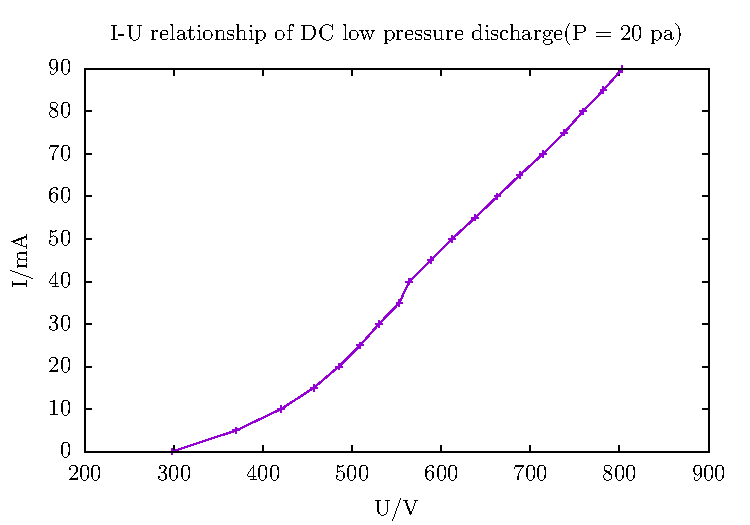
\includegraphics[width=0.9\textwidth]{./pic1_1.pdf}
        \caption{直流低压气体放电的伏安特性曲线(P = 20 pa)}
    \end{minipage}
\end{figure}

\begin{figure}[H]
    \centering
    \begin{minipage}[b]{0.9\textwidth}
        \centering
        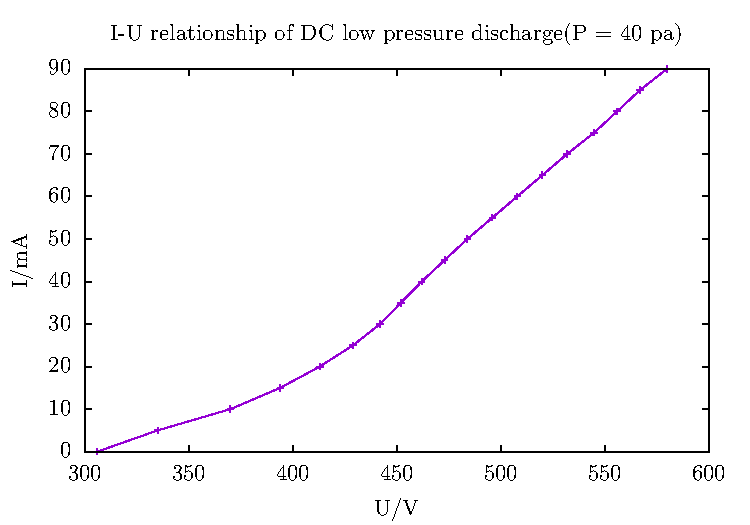
\includegraphics[width=0.9\textwidth]{./pic1_2.pdf}
        \caption{直流低压气体放电的伏安特性曲线(P = 40 pa)}
    \end{minipage}
\end{figure}

以上分别为不同气压下的直流低压气体放电的伏安特性曲线,下面将它们在同一个图中画出:

\begin{figure}[H]
    \centering
    \begin{minipage}[b]{0.9\textwidth}
        \centering
        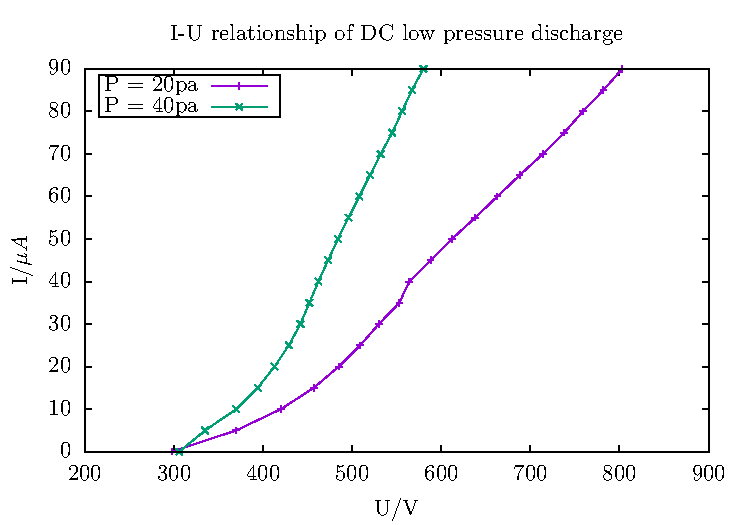
\includegraphics[width=0.9\textwidth]{./pic4.pdf}
        \caption{直流低压气体放电的伏安特性曲线}
    \end{minipage}
\end{figure}

\subsubsection{数据分析}

实验现象为:

\begin{enumerate}
    \item 当压强恒定的情况下,当电压差不多超过300V时,开始产生电流,且随着电压的增大,电流也逐渐增大。
    \item 对于相同的电压,在气压更大的时候,击穿电流也会变的更大。
\end{enumerate}

分析现象可能的原因有:

\begin{enumerate}
    \item 当电压U=300V左右为气体的击穿电压,发生从暗放电到辉光放电的转变。其中对于P=20pa时,U=298V;对于P=40pa时,U=306V。由于实验的
    误差较大(肉眼观察现象),所以最终取U=300V为击穿电压。
    \item 对于不同的气压,伏安特性曲线也不一样。在不同的气压下,气体的击穿电压相差不大,由于要产生气体的电离,电子需要到达一定的能量,对于不同气压下的气体来说,这个能量的大小是几乎确定的;在气压高的情况下$K=\frac{d\,I}{d\,U}$更大,即伏安特性曲线更陡峭。
    可能是由于在气压高的时候,气体分子的分子数密度n更大,导致更加容易发生电离,气体的导电能力变强,使得$\frac{d\,I}{d\,U}$变大。
\end{enumerate}

\subsection{气体击穿电压的测定}

\begin{figure}[H]
    \centering
    \begin{minipage}[b]{0.9\textwidth}
        \centering
        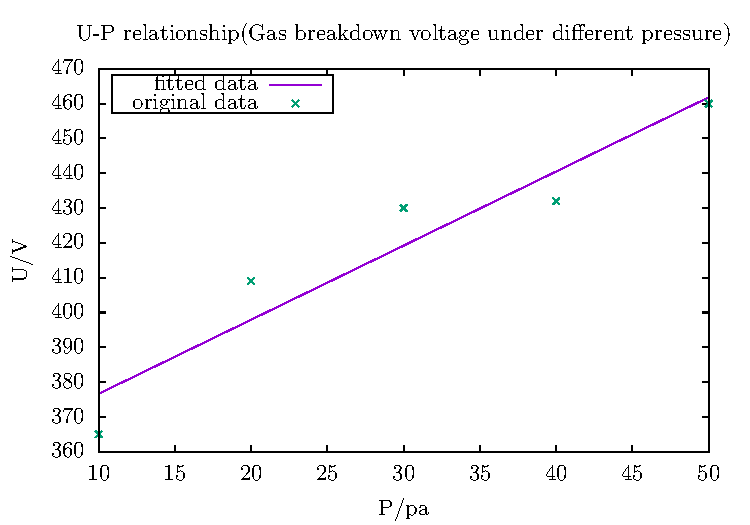
\includegraphics[width=0.9\textwidth]{./pic2.pdf}
        \caption{气体于不同击穿电压处的拟合曲线}
    \end{minipage}
\end{figure}

观察发现,随着气压的增强,气体的击穿电压也逐渐增加。说明帕邢定律中的p与$V_b$呈正相关,且其线性性不是特别良好,符合帕邢定律。

\subsection{郎缪尔双探针法测电子温度和等离子体密度}

\begin{figure}[H]
    \centering
    \begin{minipage}[b]{0.9\textwidth}
        \centering
        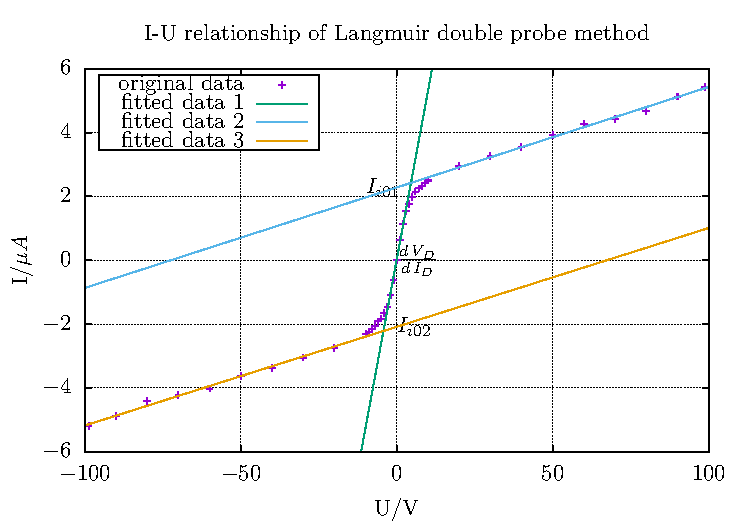
\includegraphics[width=0.9\textwidth]{./pic3.pdf}
        \caption{气体于不同击穿电压处的拟合曲线}
    \end{minipage}
\end{figure}

得到的拟合曲线方程分别为:

\begin{equation}
    I_1(\mu A) = 0.527 U(V) + 0.0214   
\end{equation}

\begin{equation}
    I_2(\mu A) = 0.0315 U(V) + 2.281
\end{equation}

\begin{equation}
    I_3(\mu A) = 0.0310 U(V) - 2.086
\end{equation}

其中$I_1,I_2,I_3$分别对应上图中的fitted data 1,fitted data 2,fitted data 3;分别取的是中心的7个电和旁边的各10个点。可得结果:

\begin{equation}
    \frac{d\,V_D}{d\,I_D}\bigg|_{V_D = 0} = \frac{1}{\frac{d\,I_D}{d\,V_D} \bigg|_{V_D = 0}} = \frac{1}{0.527\frac{\mu A}{V}} = 1.898 \times 10^6 (V/A)
\end{equation}

\begin{equation}
    I_{i01} = 2.281 \mu A, \quad I_{i02} = -2.086 \mu A, \quad \left\lvert I_{i02}\right\rvert = 2.086 \mu A
\end{equation}

由电子温度计算公式可得:

\begin{equation}
    \begin{aligned}
        T_e &= -\frac{e}{k} \frac{I_{i01}I_{i02}}{I_{i01}+I_{i02}} (\frac{d\,V_D}{d\,I_D}\bigg|_{V_D = 0}) \\ 
        &= \frac{1.602 \times 10^{-19}C}{1.381\times 10^{-23} J/K} \frac{2.281 \cdot 2.086 \cdot (10^{-6}A)^2}{(2.281+2.086) \cdot(10^{-6}A)} \cdot \frac{1.898 \times 10^6V}{A} \\
        &= 2.3998 \times 10^4 K
    \end{aligned}
\end{equation}

可计算得电子的数密度为:

\begin{equation}
    n_e = \frac{4I_{e0}}{eS_e} \sqrt{\frac{\pi m_e}{8k T_e}} = \frac{4 \cdot 0.05A}{e \cdot 0.04cm^2} \sqrt{\frac{\pi \cdot 0.91 \cdot 10^{-30}kg}{8\cdot\frac{23998}{11600}eV}} = 3.240 \times 10^{11} cm^{-3}
\end{equation}

其中,取$I_{e0} = 0.05A,S_e = 0.04cm^2$

综上,于$P_{gas}=20pa,P=8.645W$时,电子的温度$T_e = 2.3998 \times 10^4 K$,电子的数密度为$n_e = 3.24\times 10^{11} cm^{-3}$

\section{实验总结和误差分析}

\subsection{误差分析}

由于实验装置是集成的,无法分析其结构中的误差,只能给出一些测量误差和其它可能的误差。

\begin{enumerate}
    \item 在直流低压放电的实验中,用肉眼难以区分辉光消失的情况,且变化回暗放电的时候电压示数变化很快,故导致击穿电压难以确定。
    \item 在气体击穿的测定实验中,由于在击穿时刻,电压示数变化很快,且电压示数本身就存在延迟,故记录的数据存在一些误差。
    \item 在朗缪尔双探针法实验中,由于每次测量时的电流的示数会来回变化,虽然利用了估读,但还是存在误差。
\end{enumerate}

\subsection{实验总结}

\begin{enumerate}
    \item 在直流低压放电实验中,测得气体的击穿电压约为300V,且随着气压的变大,伏安特性会变得更陡峭($\frac{d\,I}{d\,U}$会变得更大)
    \item 在帕邢定律中,P与$V_b$呈正相关
    \item 计算得:于$P_{gas}=20pa,P=8.645W$时,电子的温度$T_e = 2.3998 \times 10^4 K$,电子的数密度为$n_e = 3.24\times 10^{11} cm^{-3}$
\end{enumerate}

\section{思考题}

\subsection{暗放电区电流的测量应注意什么问题?}

由于暗放电时,其击穿电流的范围为$10^{-5}$-$10^{-10}A$,且由于升降电压方向不同,会导致不同的物理情况,所以取测量范围为$10^{-7}$-$10^{-10}$时测量的结果比较精确。
由于其电流较小,故直接测量误差会很大,通常使用电压求电流。且测量电路的阻抗应该尽可能地大,以避免因电路负载过重而影响测量结果。

\subsection{阴极与阳极显著的热效应差别的原因?}

在直流辉光放电中,电子从阴极发射出来,在电场的作用下加速,最终撞击到阳极上。在这个过程中,电子会失去一部分能量,这些能量会以热的形式释放出来。由于阴极表面的电子密度高,因此阴极受到的电子撞击更加频繁和强烈,产生的热效应也更显著。

另一方面,阳极表面的电子密度较低,因此阳极受到的电子撞击比较稀疏和弱,产生的热效应也相对较小,因此它能够更好地承受电子撞击产生的热效应。

\subsection{磁场和工作气压对辉光放电中的 V-A 特性曲线有何影响?其影响机制是什么?
(选做)}

\begin{enumerate}
    \item 加入磁场后,电子还会受狭义上的洛伦兹力的作用。
    加入磁场可以改变电子的运动轨迹和速度,从而影响电子的能量损失和电流密度分布。当磁场增加时,电子的运动轨迹变得更加弯曲,电子与气体分子的碰撞概率也增加,因此电子在单位长度内的能量损失增加,电流密度也会随之增加。这会导致V-A特性曲线向上弯曲,并且在较低电压下就可以观察到较高的电流。
    \item 气压的变化会影响气体的电离和激发过程,从而影响电流密度和电压的分布。当气压增加时,气体分子的密度增加,电离和激发过程的概率也增加,因此电子在单位长度内的能量损失也会增加,电流密度也会随之增加。这会导致V-A特性曲线向上弯曲,并且在较低电压下就可以观察到较高的电流。
\end{enumerate}

\end{document}